\documentclass[conference]{IEEEtran}
\IEEEoverridecommandlockouts
% The preceding line is only needed to identify funding in the first footnote. If that is unneeded, please comment it out.
\usepackage{cite}
\usepackage{hyperref}
\usepackage{amsmath,amssymb,amsfonts}
\usepackage{algorithmic}
\usepackage{graphicx}
\usepackage{textcomp}
\usepackage{listings}
\lstset{
  basicstyle=\ttfamily,
  breaklines=true,
  postbreak=\mbox{\textcolor{red}{$\hookrightarrow$}\space},
}


\usepackage{xcolor}
\def\BibTeX{{\rm B\kern-.05em{\sc i\kern-.025em b}\kern-.08em
    T\kern-.1667em\lower.7ex\hbox{E}\kern-.125emX}}
\begin{document}

\title{Implementing Deep Learning Models for Enhancing Bluetooth-based Localization Algorithms*\\
{\footnotesize \textsuperscript{*}Advances in Indoor Localization Using Deep Learning Techniques}
\thanks{Identify applicable funding agency here. If none, delete this.}
}

\author{\IEEEauthorblockN{1\textsuperscript{st} Camilo Leuro}
\IEEEauthorblockA{\textit{dept. Ciencias de la Computación e IA} \\
\textit{Universidad Sergio Arboleda}\\
Bogotá, Colombia \\
camilo.leuro01@usa.edu.co}
\and
\IEEEauthorblockN{2\textsuperscript{nd} Carolay Camacho-Sanchez}
\IEEEauthorblockA{\textit{dept. Ciencias de la Computación e IA} \\
\textit{Universidad Sergio Arboleda}\\
Bogotá, Colombia \\
carolay.camacho01@usa.edu.co}
\and
\IEEEauthorblockN{3\textsuperscript{rd} Andrés García}
\IEEEauthorblockA{\textit{dept. Ciencias de la Computación e IA} \\
\textit{Universidad Sergio Arboleda}\\
Bogotá, Colombia \\
andres.garcia13@usa.edu.co}
\and
\IEEEauthorblockN{4\textsuperscript{th} Mateo Rondon}
\IEEEauthorblockA{\textit{dept. Ciencias de la Computación e IA} \\
\textit{Universidad Sergio Arboleda}\\
Bogotá, Colombia\\
mateo.rondon01@usa.edu.co}
}

\maketitle

\begin{abstract}
Indoor localization remains a challenge in the absence of reliable GPS signals. This study addresses this issue using advanced Deep Learning techniques. We employ the UJIIndoorLoc dataset to construct a model based on WLAN fingerprinting, executed within a Python programming environment and following the CRISP-DM methodology. Our findings underscore the pivotal role of deep learning in addressing indoor localization challenges, offering promising solutions for real-world applications.
\end{abstract}

\begin{IEEEkeywords}
Indoor localization, UJIIndoorLoc, Wireless fingerprinting, Data analysis.
\end{IEEEkeywords}

\maketitle


\section{Introduction}
The relentless progress of technology continually shapes and redefines our interaction with the world around us. Among the many technological evolutions, indoor localization stands out as a game-changer, with the potential to aid individuals in vast shopping malls, ensure patient safety in hospitals, and assist travelers in international airports. Despite historical attempts using solutions ranging from infrared to ultrasonic sensors, achieving reliable indoor localization remains challenging. The limitations of the Global Positioning System (GPS) in indoor environments due to architectural barriers intensify this challenge. In this milieu, the rise of Deep Learning, with its ability to decipher patterns from extensive datasets, promises potential breakthroughs. Leveraging the rich data from the UJIIndoorLoc dataset and following the CRISP-DM methodology, this study explores the intricacies of indoor positioning, aiming to make a significant contribution in the domain of Deep Learning applications.

Our specific objectives include:
\begin{enumerate}
\item Constructing a WLAN fingerprint-based model using the UJIIndoorLoc dataset.
\item Implementing the research within a Python programming framework.
\item Following the CRISP-DM methodology to ensure a structured and comprehensive approach.
\item Highlighting the pivotal role of Deep Learning in offering promising solutions to the challenges of indoor localization.
\end{enumerate}


\section{Literature Review}

The domain of indoor localization has garnered considerable attention in recent times, propelled by the pressing need for accurate positioning in environments where traditional GPS signals are elusive. A pivotal contribution in this arena comes from Terán and Ore, who in 2019 embarked on a meticulous exploration of the UJIIndoorLoc dataset, benchmarking various algorithms designed for discerning user indoor positioning \textcolor{blue}{\cite{teran2019benchmark}}. This seminal work by Terán and Ore not only elucidated the nuances of the dataset but also proffered a nuanced understanding of the strengths and potential pitfalls of several algorithms. Their findings serve as a touchstone for subsequent research endeavors, facilitating a deeper appreciation of the intricacies associated with indoor positioning.

Complementing this research trajectory, the domain has seen a burgeoning interest in leveraging deep learning techniques for indoor localization, especially within the paradigm of WiFi fingerprinting. In their study, Alsheikh et al. (2015) extolled the virtues of deep learning, emphasizing its profound capability to model intricate relationships, thereby amplifying positioning accuracy\textcolor{blue}{\cite{alsheikh2015deep}}. Such findings underscore the transformative potential of deep learning techniques in surmounting the myriad challenges endemic to indoor localization.

Zhang et al.'s comprehensive review in 2013 further amplifies our understanding of the multifaceted nature of technologies underpinning indoor localization\textcolor{blue}{\cite{zhang2013comprehensive}}. By delineating the evolution of various technologies, from the erstwhile infrared and ultrasonic sensors to the avant-garde methodologies, Zhang et al. provide invaluable insights into the trajectory of indoor positioning systems.

Taken in concert, these studies weave a rich tapestry of insights and findings in the realm of indoor localization. The pioneering work of researchers like Marco A. Terán plays an instrumental role in shaping this landscape, providing both direction and impetus for future investigations. As we navigate the complex terrain of the UJIIndoorLoc dataset in our current study, the foundational work of Terán and others serves as both a beacon and a guidepost.

\section{Dataset Description}

The dataset under scrutiny is the \textbf{UJIIndoorLoc}, meticulously curated by Joaquín Torres-Sospedra and collaborators\textcolor{blue}{\cite{UJIIndoorLocPap}}. This dataset offers a deep dive into the realm of indoor positioning systems, primarily focusing on WLAN fingerprinting or WiFi Fingerprinting. Created based on data captured in 2013 from 3 buildings with 3 and 4 floors of the Universitat Jaume I, it embodies the nuances and intricacies of indoor localization.

A holistic breakdown of its components is as follows:

\begin{itemize}
\item \textbf{Attributes 001 to 520 (WAP001-WAP520):} These delineate the intensity values from various Wireless Access Points (WAP). The values extend from $-104$ to $0$ and $+100$. It's noteworthy that a positive value of $100$ indicates non-detection of the WAP.
\item \textbf{Longitude:} Represents longitudinal coordinates, varying from -7695.9387549299299000 to -7299.786516730871000.
\item \textbf{Latitude:} Parallelly, latitude coordinates span from 4864745.7450159714 to 4865017.3646842018.
\item \textbf{Floor:} Specifies the altitude in terms of the building's floors, capturing integer values between 0 to 4.
\item \textbf{BuildingID:} A categorical indicator segregating the buildings. It assumes integer values from 0 to 2.
\item \textbf{SpaceID:} A categorical value illustrating the precise space (be it an office, corridor, classroom) of data capture.
\item \textbf{RelativePosition:} Portrays the positional nuance concerning the space, either being inside (1) or outside in front of the door (2).
\item \textbf{User ID, PhoneID, and Timestamp:} These attributes offer additional metadata about the user, the Android device used for data collection, and the exact UNIX timestamp of the data capture, respectively.
\end{itemize}

In terms of data typology, all attributes are instantiated as int64, barring longitude and latitude, which are represented as float64.

The \textbf{UJIIndoorLoc} dataset is a paragon in the sphere of indoor positioning. In light of the hitches posed by GPS systems in interior spaces due to architectural barriers, the gravity of precise indoor positioning stands unparalleled. Harnessing the unique signatures of proximate WiFi access points (WAPs) for device localization, this dataset accentuates the prowess of WiFi fingerprinting. The gamut of data, spanning WAP intensities, precise geospatial data, floor details, and building categorization, fortifies the dataset's primacy in advancing accurate indoor positioning—rendering it indispensable for aficionados and trailblazers in the field.

\section{Data Processing and Analysis}

In order to derive meaningful insights from the \textbf{UJIIndoorLoc} dataset, meticulous data processing and analysis were conducted. This encompassed preprocessing, exploratory data analysis, feature selection, and model implementation, ensuring that the data was molded into a format apt for high-quality insights.

\begin{enumerate}
\item \textbf{Preprocessing:} Initial procedures included managing missing data, normalizing intensity values to bring them onto a common scale, and encoding categorical variables. The aim was to refine the dataset by addressing any inconsistencies or discrepancies, setting it up for further analysis.


\item \textbf{Exploratory Data Analysis (EDA):} This phase sought to uncover underlying patterns, correlations, and outliers in the dataset. Visualization techniques and statistical approaches were utilized to understand the dataset's attributes, illuminating key elements for subsequent feature selection.

\item \textbf{Feature Selection:} Based on the revelations from the EDA, essential features were chosen to enhance the model's efficiency. This step concentrated on diminishing dimensionality, removing superfluous or redundant features, and preserving those with significant contributions to the model's predictive prowess.

\item \textbf{Model Implementation:} After feature selection, a variety of machine learning models were trialed and assessed based on their performance indicators. The best-performing model was further refined and validated to ensure it aptly captured the intricacies of indoor positioning.
\end{enumerate}

By systematically navigating through these phases, the \textbf{UJIIndoorLoc} dataset was elevated to a powerful instrument, primed to decode the complexities of indoor positioning. The refined dataset, equipped with enhanced features and a formidable model, showcases the progress in indoor positioning technologies and stands as a pivotal resource for ongoing research and advancements in the sector.



\subsection{Description of the CRISP Methodology}
\label{sec:metodo_crisp}

The Cross Industry Standard Process for Data Mining (CRISP-DM) served as the foundational methodology guiding our exploration of the \textbf{UJIIndoorLoc} dataset. This iterative process consists of six essential stages, which were meticulously applied and adapted to the intricacies of indoor positioning data. The stages and their specific applications to our dataset are described below:

\begin{enumerate}
    \item \textbf{Understanding the Business:} At this stage, our primary objective was to comprehend the challenges associated with indoor positioning, especially in environments where GPS signals are ineffective. Our goal was to harness the capabilities of the \textbf{UJIIndoorLoc} dataset to address these challenges.
    
    \item \textbf{Understanding the Data:} A comprehensive exploration of the dataset was conducted, discerning attributes like intensity values from different WAPs, geospatial data, floor numbers, and building identifiers. This step was crucial to appreciate the dataset's potential in addressing indoor positioning needs.
    
    \item \textbf{Data Preparation:} The data was scrutinized for missing values, inconsistencies, and discrepancies. Intensity values were normalized, and categorical variables, such as the BuildingID, were appropriately encoded to prepare the dataset for modeling.
    
    \item \textbf{Modeling:} Based on the insights from the preliminary stages, several machine learning models were implemented. These models aimed to exploit the dataset's features to predict precise indoor positions.
    
    \item \textbf{Evaluation:} Each model's performance was rigorously assessed against predefined metrics. This evaluation was crucial in selecting the most suitable model that aligned with our business objectives and delivered optimal results for indoor positioning.
    
    \item \textbf{Implementation:} The finalized model was integrated into a suitable platform, ensuring that stakeholders could seamlessly access and utilize the results for their specific indoor positioning needs.
\end{enumerate}

By adhering to the CRISP-DM methodology, we ensured a systematic and thorough exploration of the \textbf{UJIIndoorLoc} dataset, transforming it into a valuable tool for advancing indoor positioning technologies.

\section{Visual Representation of Findings}

In this section, we delve into the UJIIndoorLoc dataset's graphical interpretations. By highlighting the specifics of WLAN fingerprinting and indoor positioning through visuals, we endeavor to bring forth patterns, correlations, and key details that might elude textual or tabular formats. Presented hereafter are a collection of visual results, each revealing distinct aspects of our detailed examination.



\begin{figure}[h!]
    \centering
    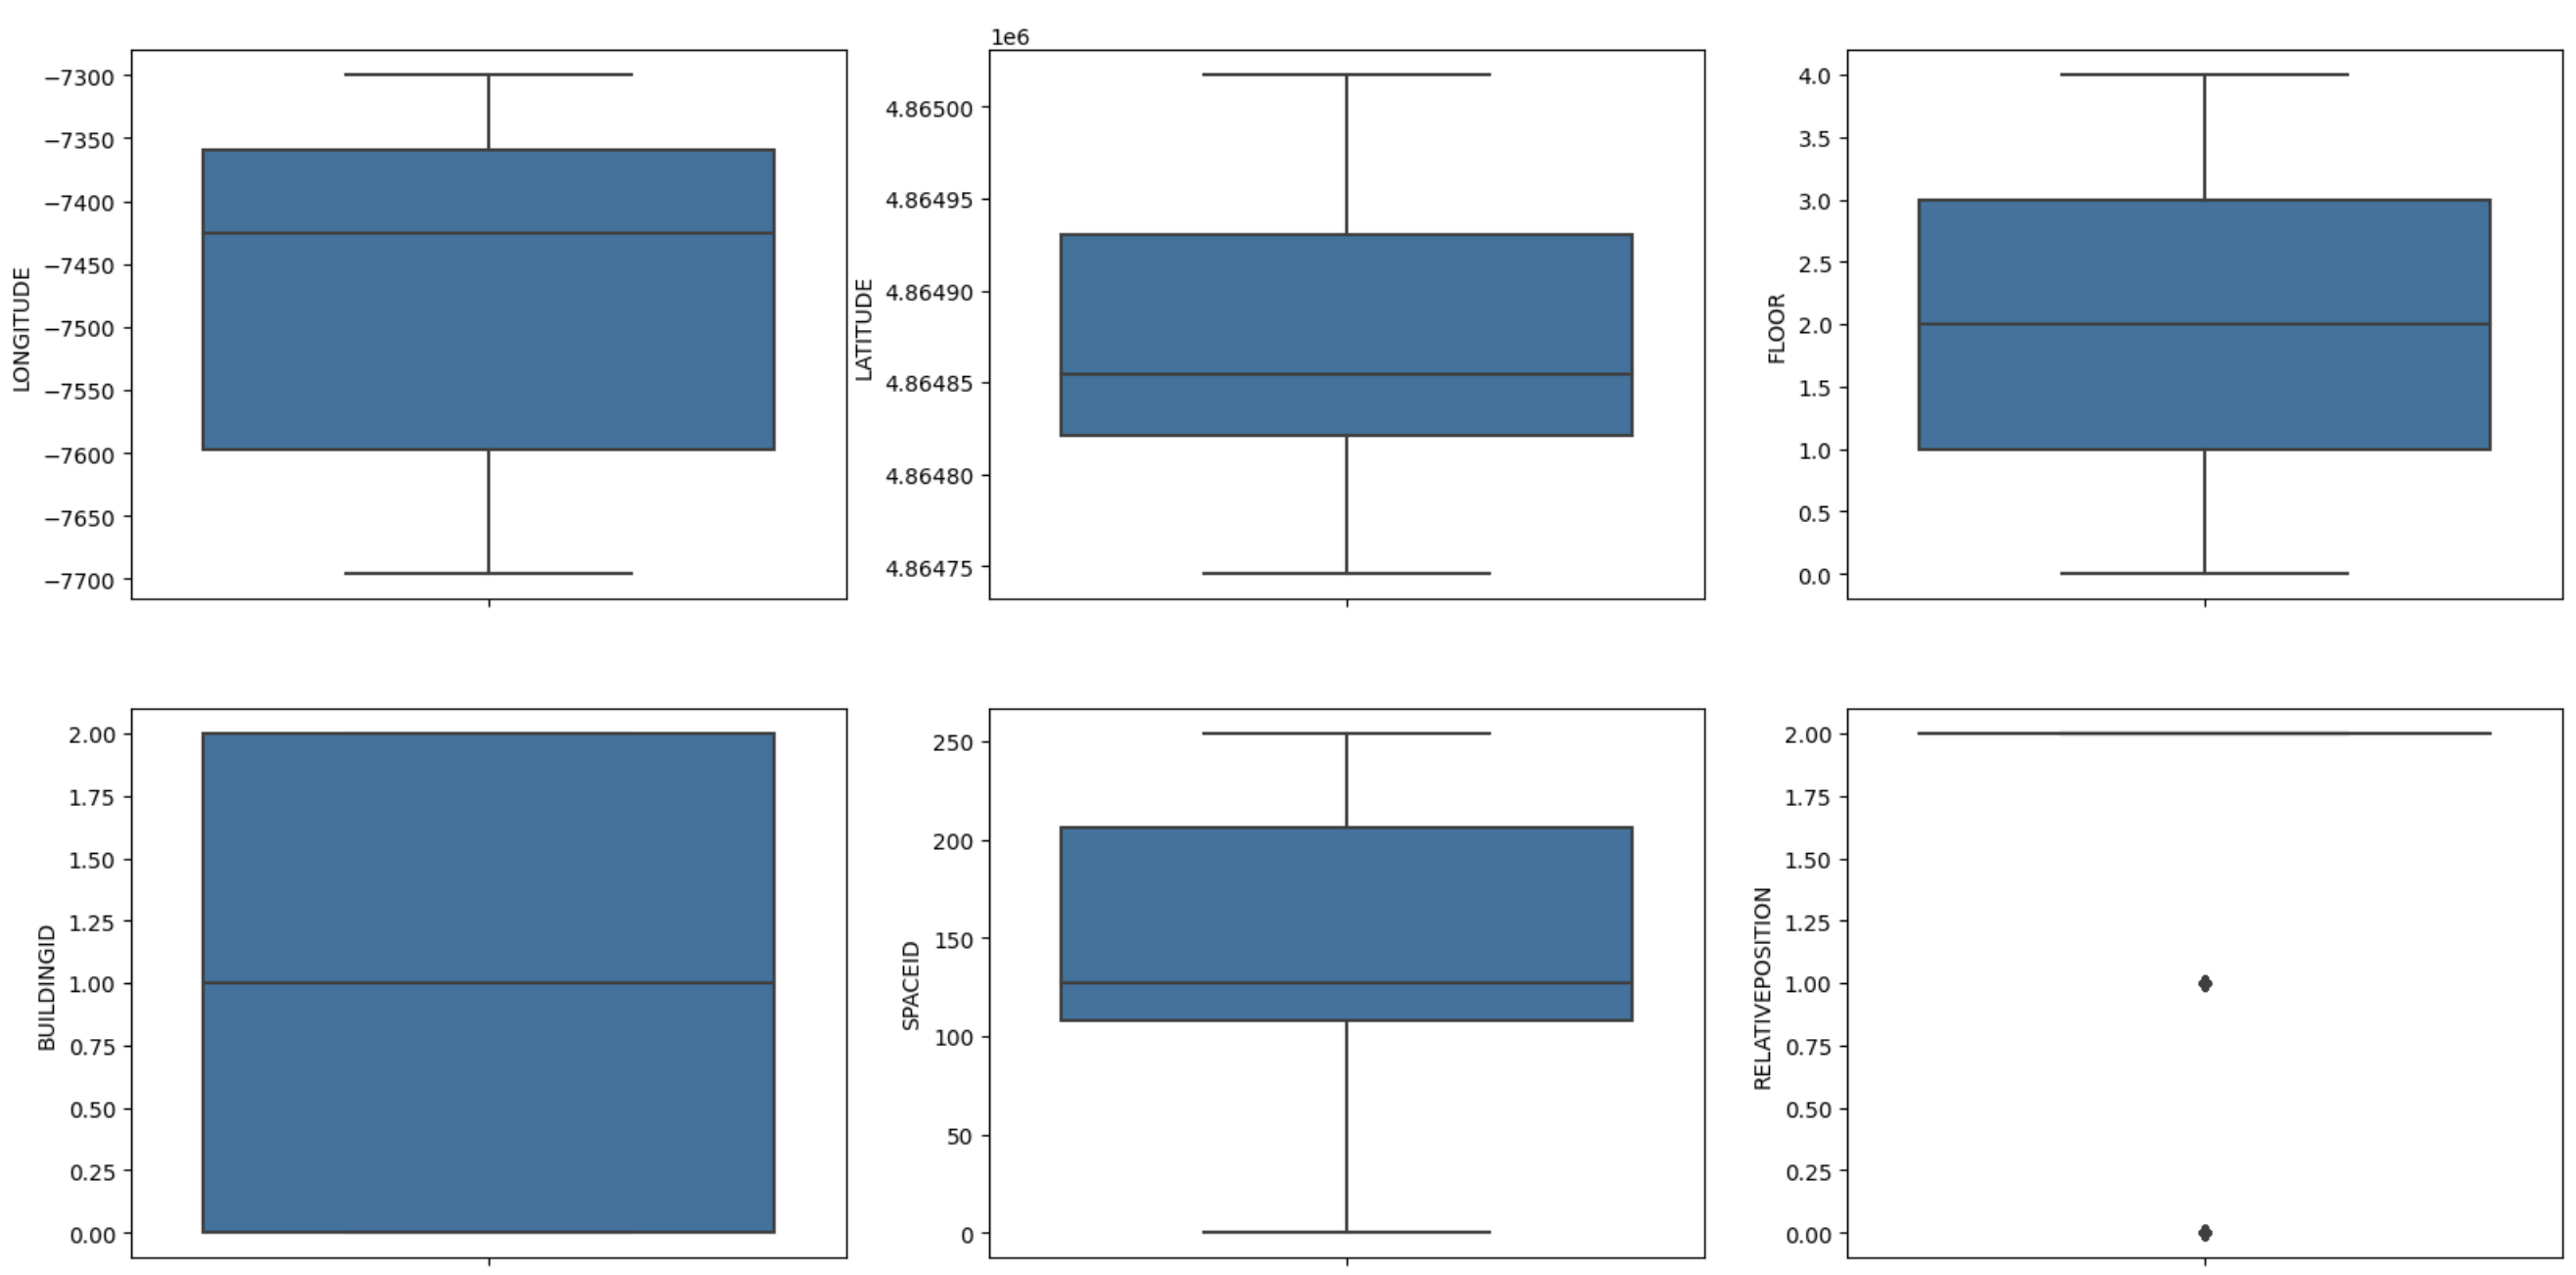
\includegraphics[width=0.5\linewidth]{Images/Figure1.png}
    \caption{Box plots for selected attributes from the UJIIndoorLoc dataset}
    \label{fig:boxplots}
\end{figure}


Figure 1 From these box plots, it is evident that within the non-intensity measurement columns, no outliers or atypical data points are observed.


\begin{figure}[h!]
    \centering
    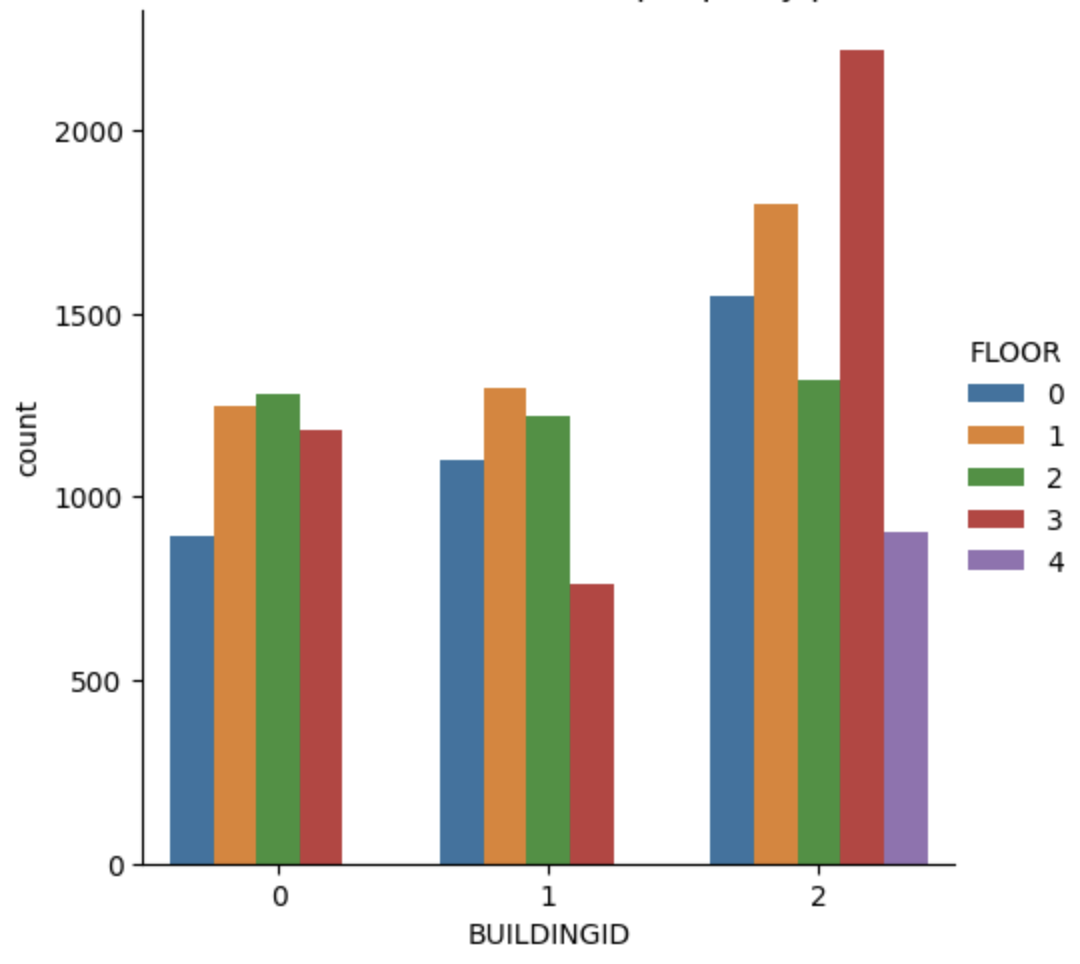
\includegraphics[width=0.5\linewidth]{Images/Imagen2.png}
    \caption{Quantity of data collected per floor and per building}
    \label{fig:enter-label}
\end{figure}


As observed in Figure 2, only one building has measurements on the 4th floor, while the others lack this, possibly due to the absence of a fourth floor.

\begin{figure}[h!]
    \centering
    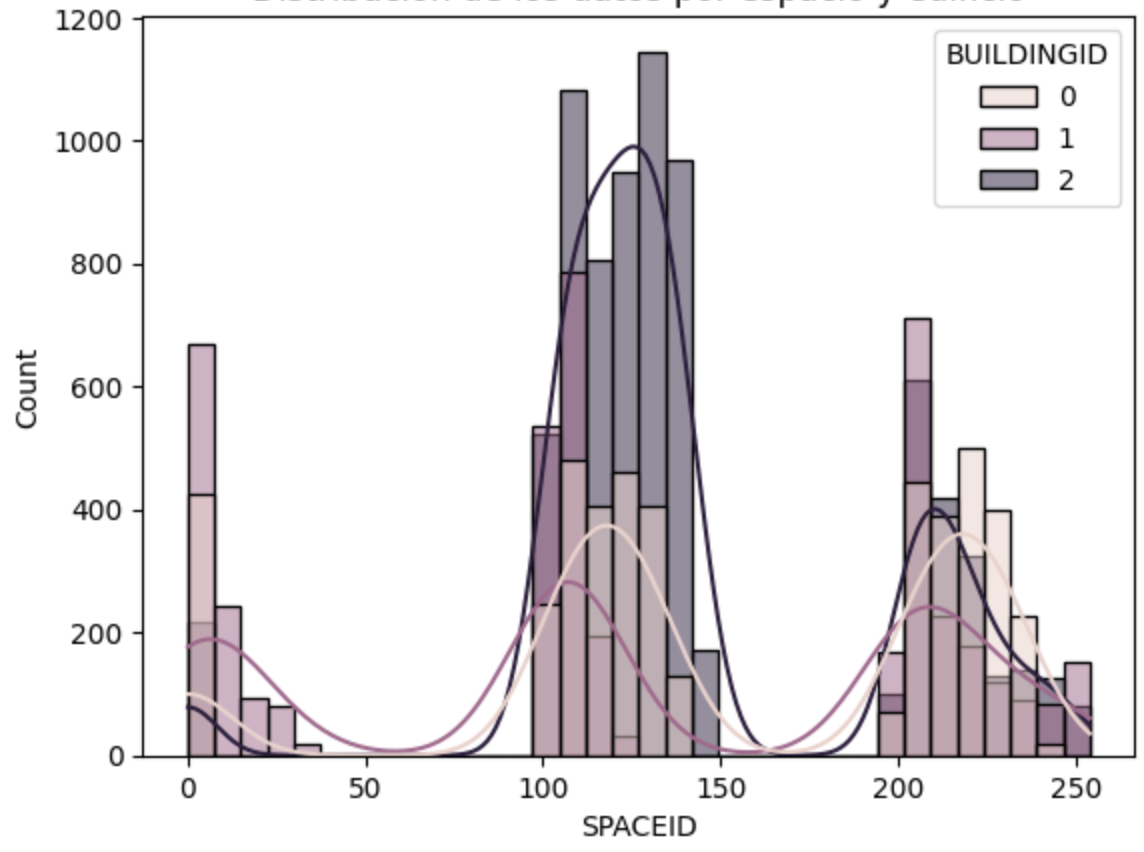
\includegraphics[width=0.5\linewidth]{Images/Image3.png}
    \caption{Distribution of data by space and building}
    \label{fig:enter-label}
\end{figure}

As depicted in Figure 3, the majority of data points are concentrated between spaces 100 to 150, with the second most prominent range being spaces 200 to 250. There is no linear categorization of spaces.


\begin{figure}[h!]
    \centering
    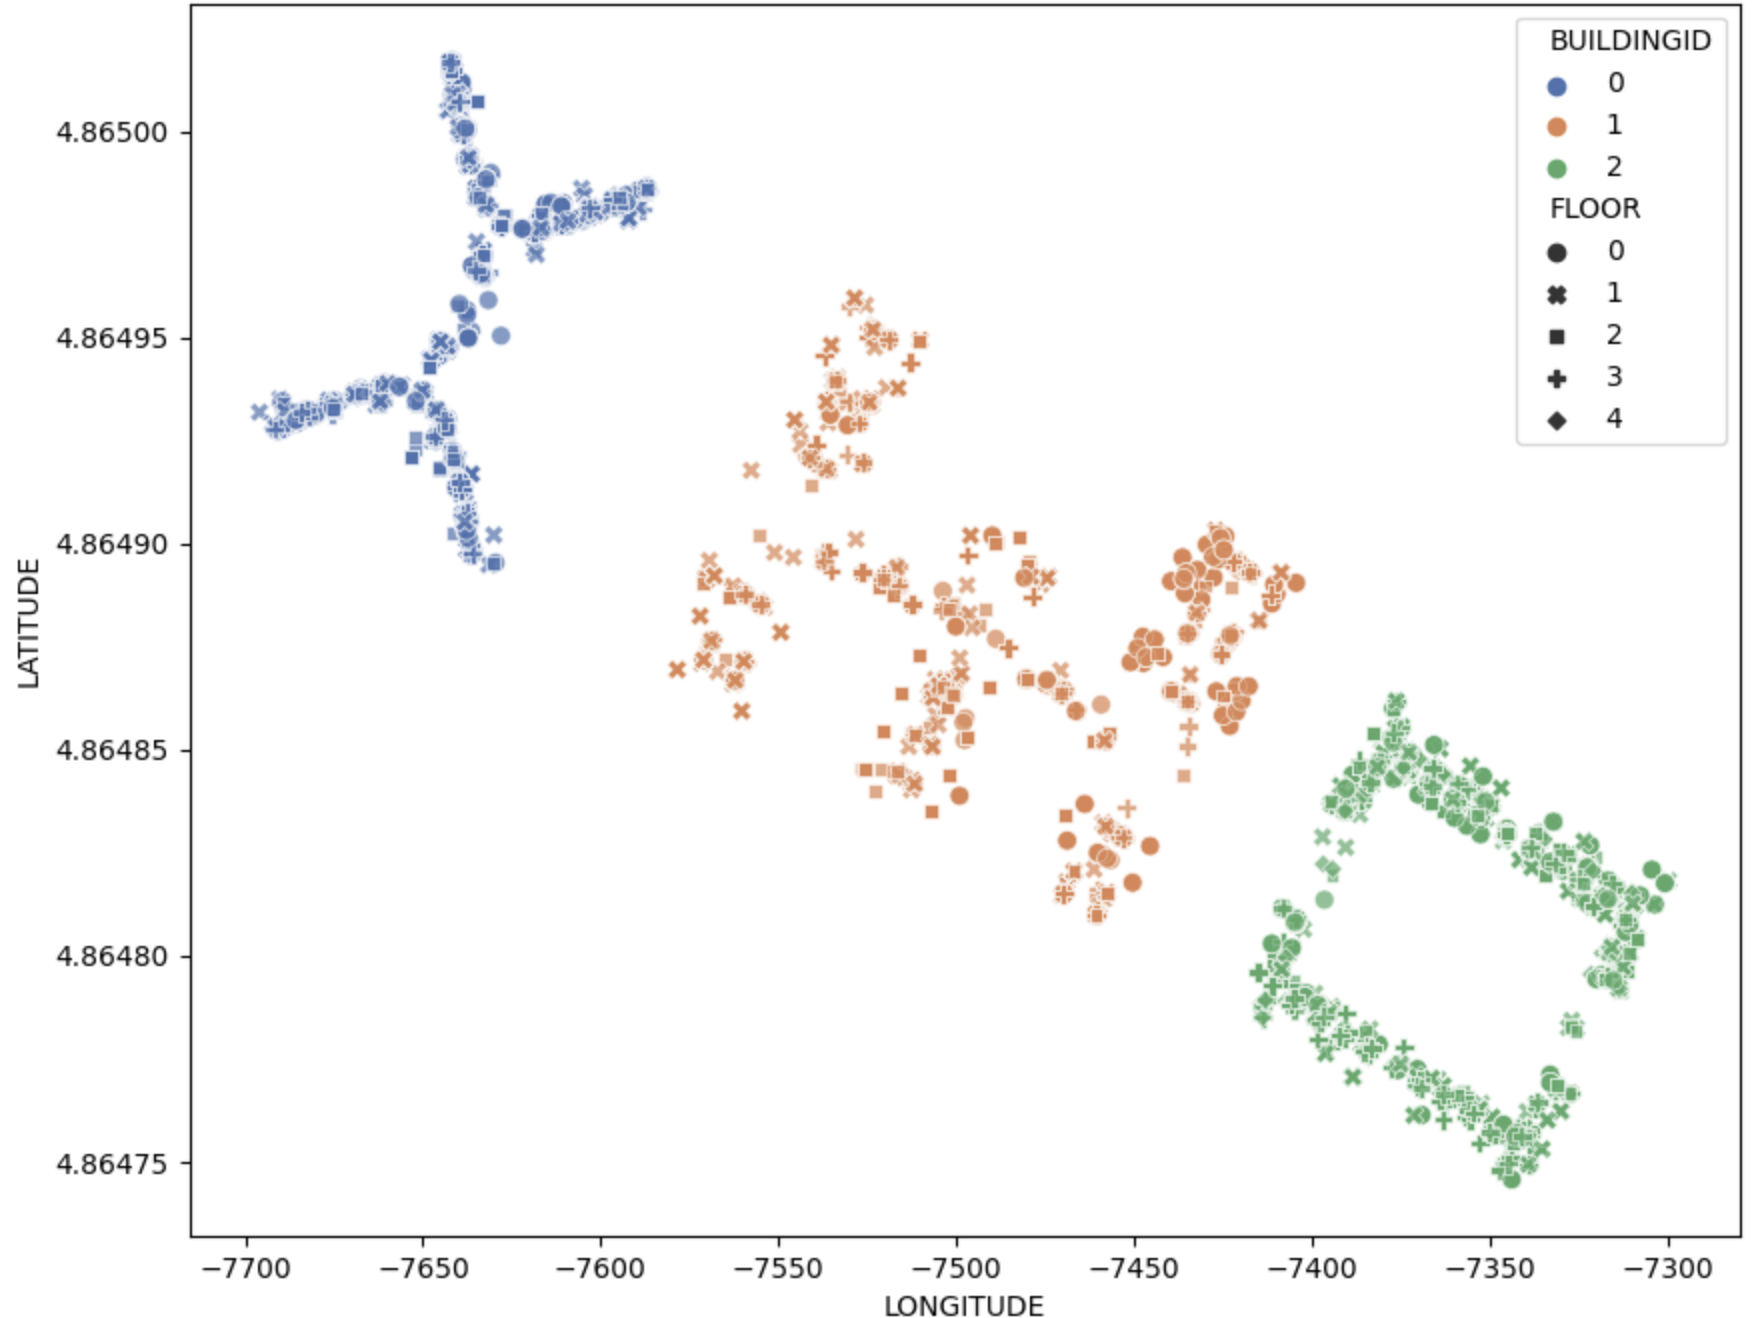
\includegraphics[width=0.5\linewidth]{Images/Figure4.png}
    \caption{Geographical Distribution of Measurements by Building and Floor}
    \label{fig:enter-label}
\end{figure}


Then, we created a series of heatmaps to visualize the average signal strength of Wireless Access Points (WAPs) across different floors. Each heatmap represents a specific floor, with columns corresponding to individual WAPs. The color scale indicates signal intensity (in dBm), where warmer colors signify stronger signals.

Notably, on the 4th floor, many attributes exhibit an average value of 100, primarily because only one building in the dataset has 4 floors. This renders several WAPs irrelevant for this floor's measurements.

Moreover, when examining specific WAPs (e.g., WAP205 to WAP221), it becomes apparent that they have limited measurements across all 4 floors, suggesting their potential insignificance for the indoor positioning model due to sparse data.

\begin{figure}[h!]
    \centering
    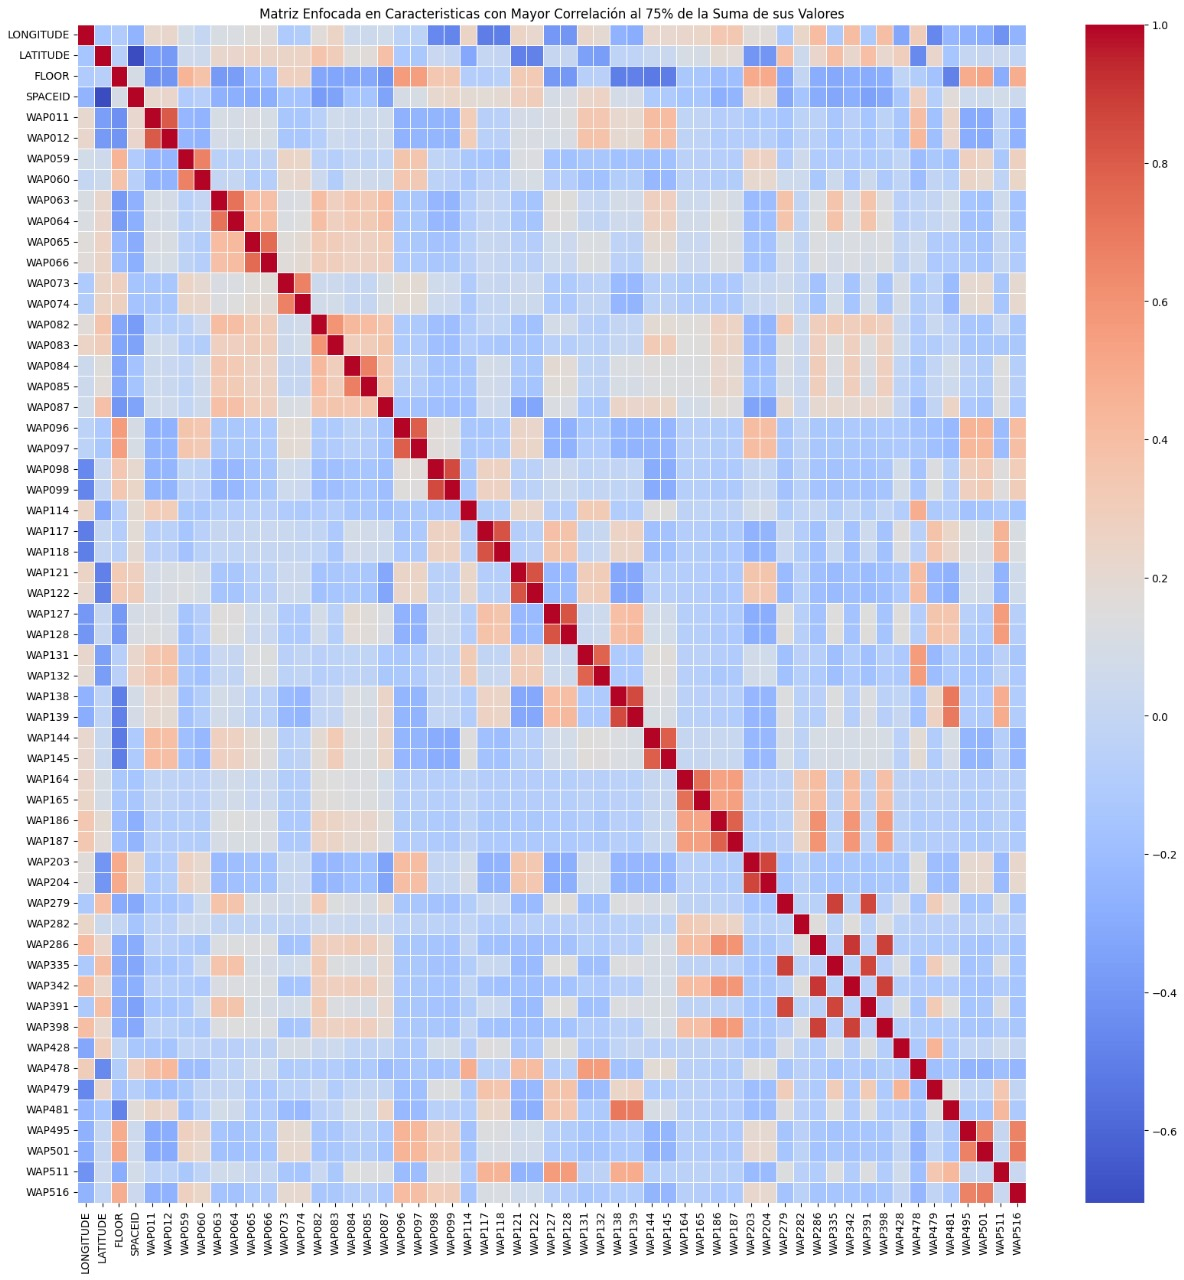
\includegraphics[width=0.5\linewidth]{Images/Imagecorrelacion.jpeg}
    \caption{Focused Matrix on Features with Higher Correlation to the Mean Sum of their Values}
    \label{fig:enter-label}
\end{figure}



Also, we constructed a correlation matrix to assess relationships between dataset attributes. The heatmap visualizes correlations, with warmer hues indicating positive correlations and cooler hues indicating negative ones. While numerical annotations are omitted for simplicity, this visualization helps identify potential patterns and associations among variables.

To narrow down our feature set for modeling, we identified columns whose cumulative correlations with other variables exceeded the average sum of all such correlations. This approach retains attributes likely to provide significant contributions to our model.

This process reduced the dataset to a subset of columns, streamlining data for modeling while maintaining data quality and relevance. The resulting dataset contains fewer columns, enhancing model development feasibility and potential accuracy for indoor positioning.


Next, we narrow our focus to a single building for in-depth analysis. We utilize box plots to visualize the distribution of selected attributes within this building. These box plots help us identify any outliers or atypical data points, particularly in non-intensity measurement columns. Fortunately, no such outliers were found in these columns.

We proceed by examining the distribution of data points across different spaces within the chosen building using a histogram. The histogram reveals that the majority of data points are concentrated within spaces numbered from 100 to 150, with the next most prominent range being spaces from 200 to 250. This distribution demonstrates the absence of a linear categorization for these spaces.

Additionally, we visualize the geographical distribution of measurements within the selected building and across different floors. The scatterplot offers insights into the building's shape based on the recorded readings.

Subsequently, we reiterate the importance of feature selection based on cumulative correlations and discuss the reduction in the number of columns. 

\begin{figure}[h!]
    \centering
    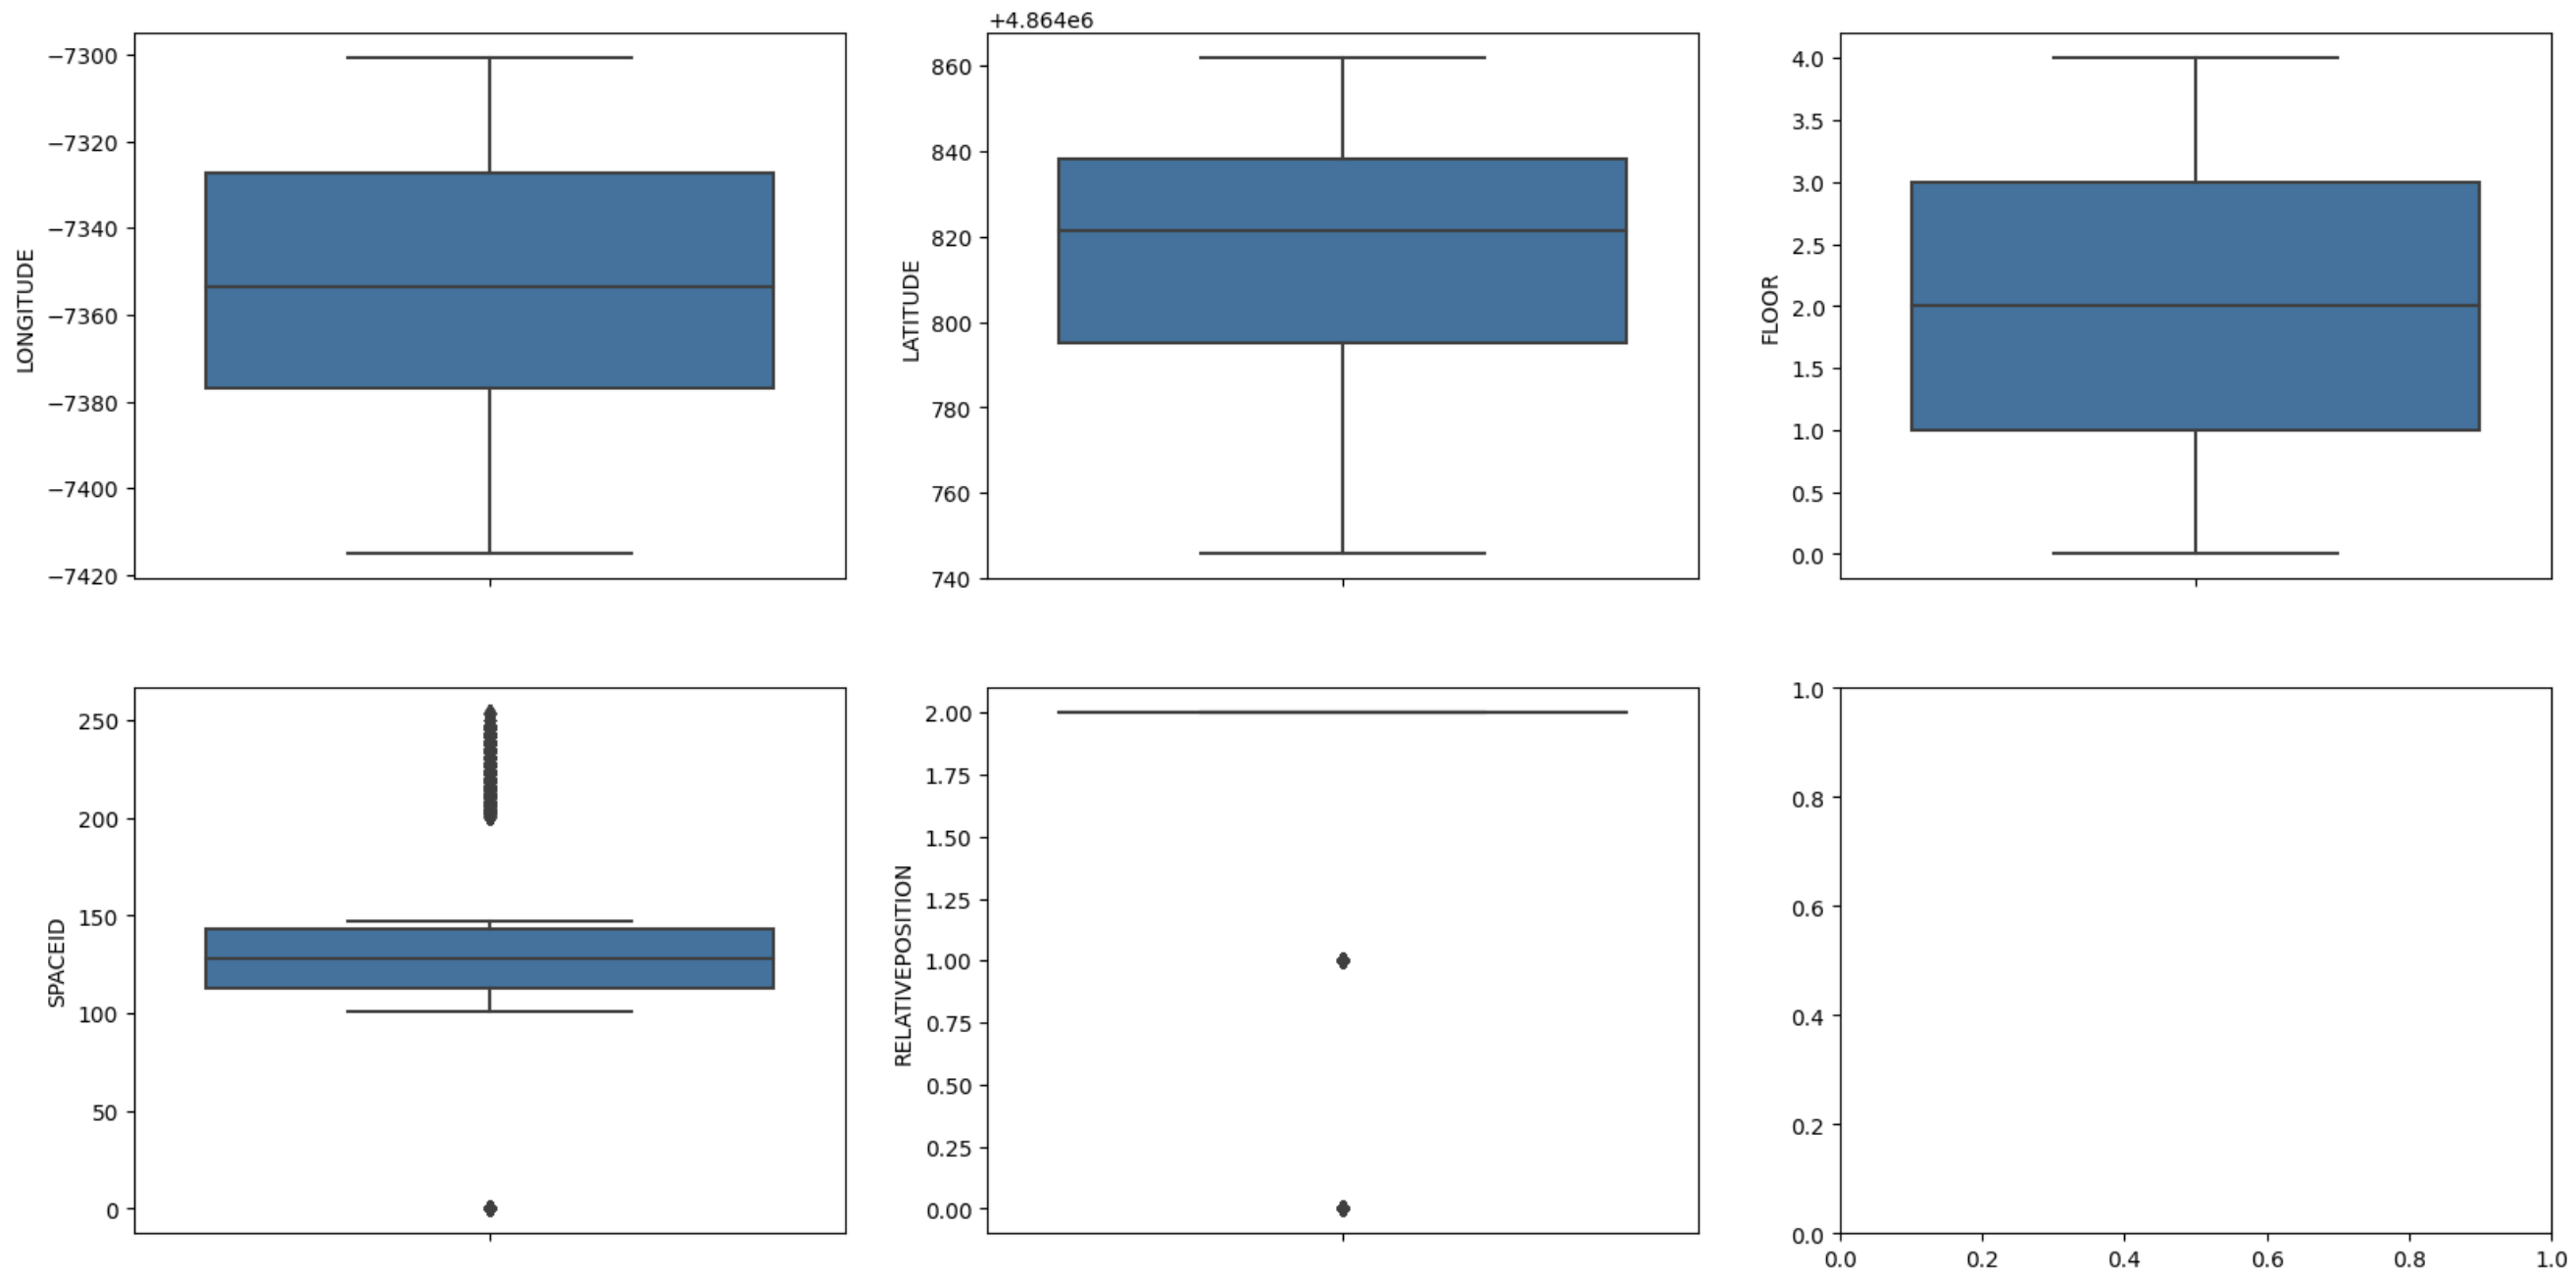
\includegraphics[width=0.5\linewidth]{Images/image5.png}
    \caption{Box Plots for Attribute Distribution}
    \label{fig:enter-label}
\end{figure}

\begin{figure}[h!]
    \centering
    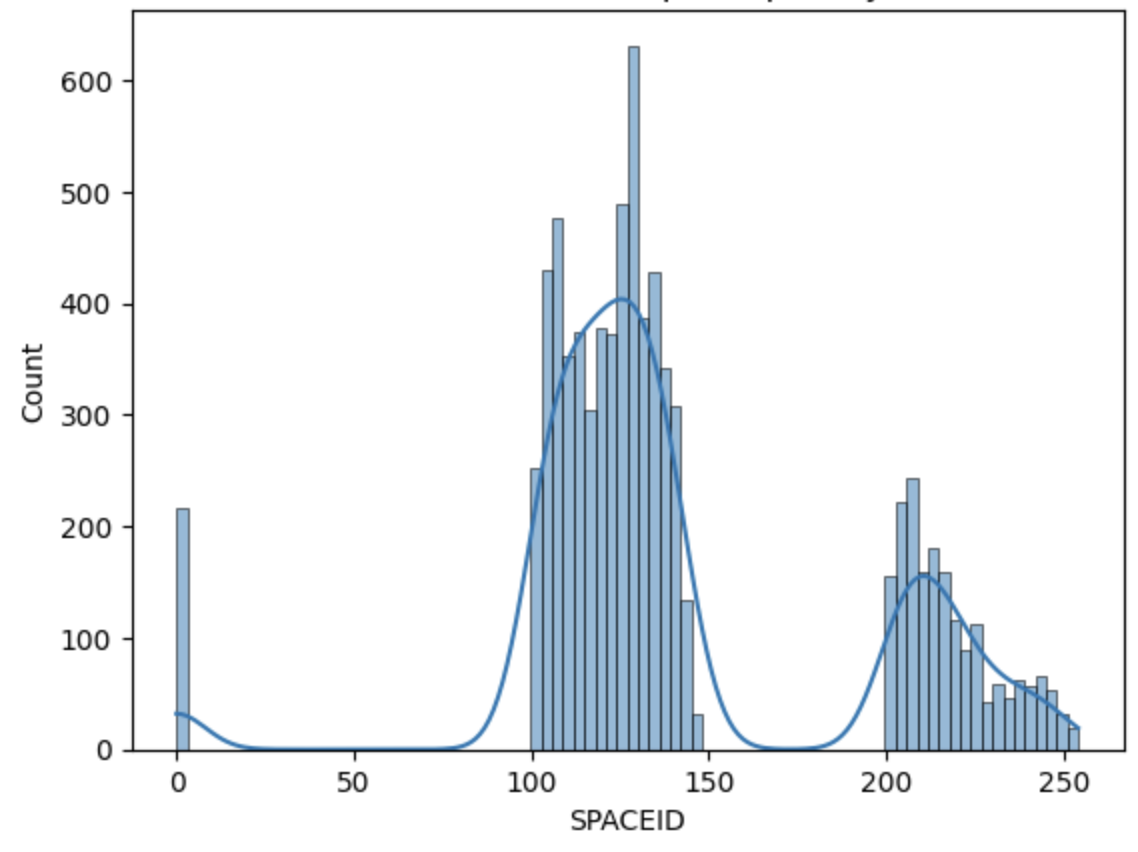
\includegraphics[width=0.5\linewidth]{Images/Image6.png}
    \caption{Data Distribution by Space and Building}
    \label{fig:enter-label}
\end{figure}

\begin{figure}[h!]
    \centering
    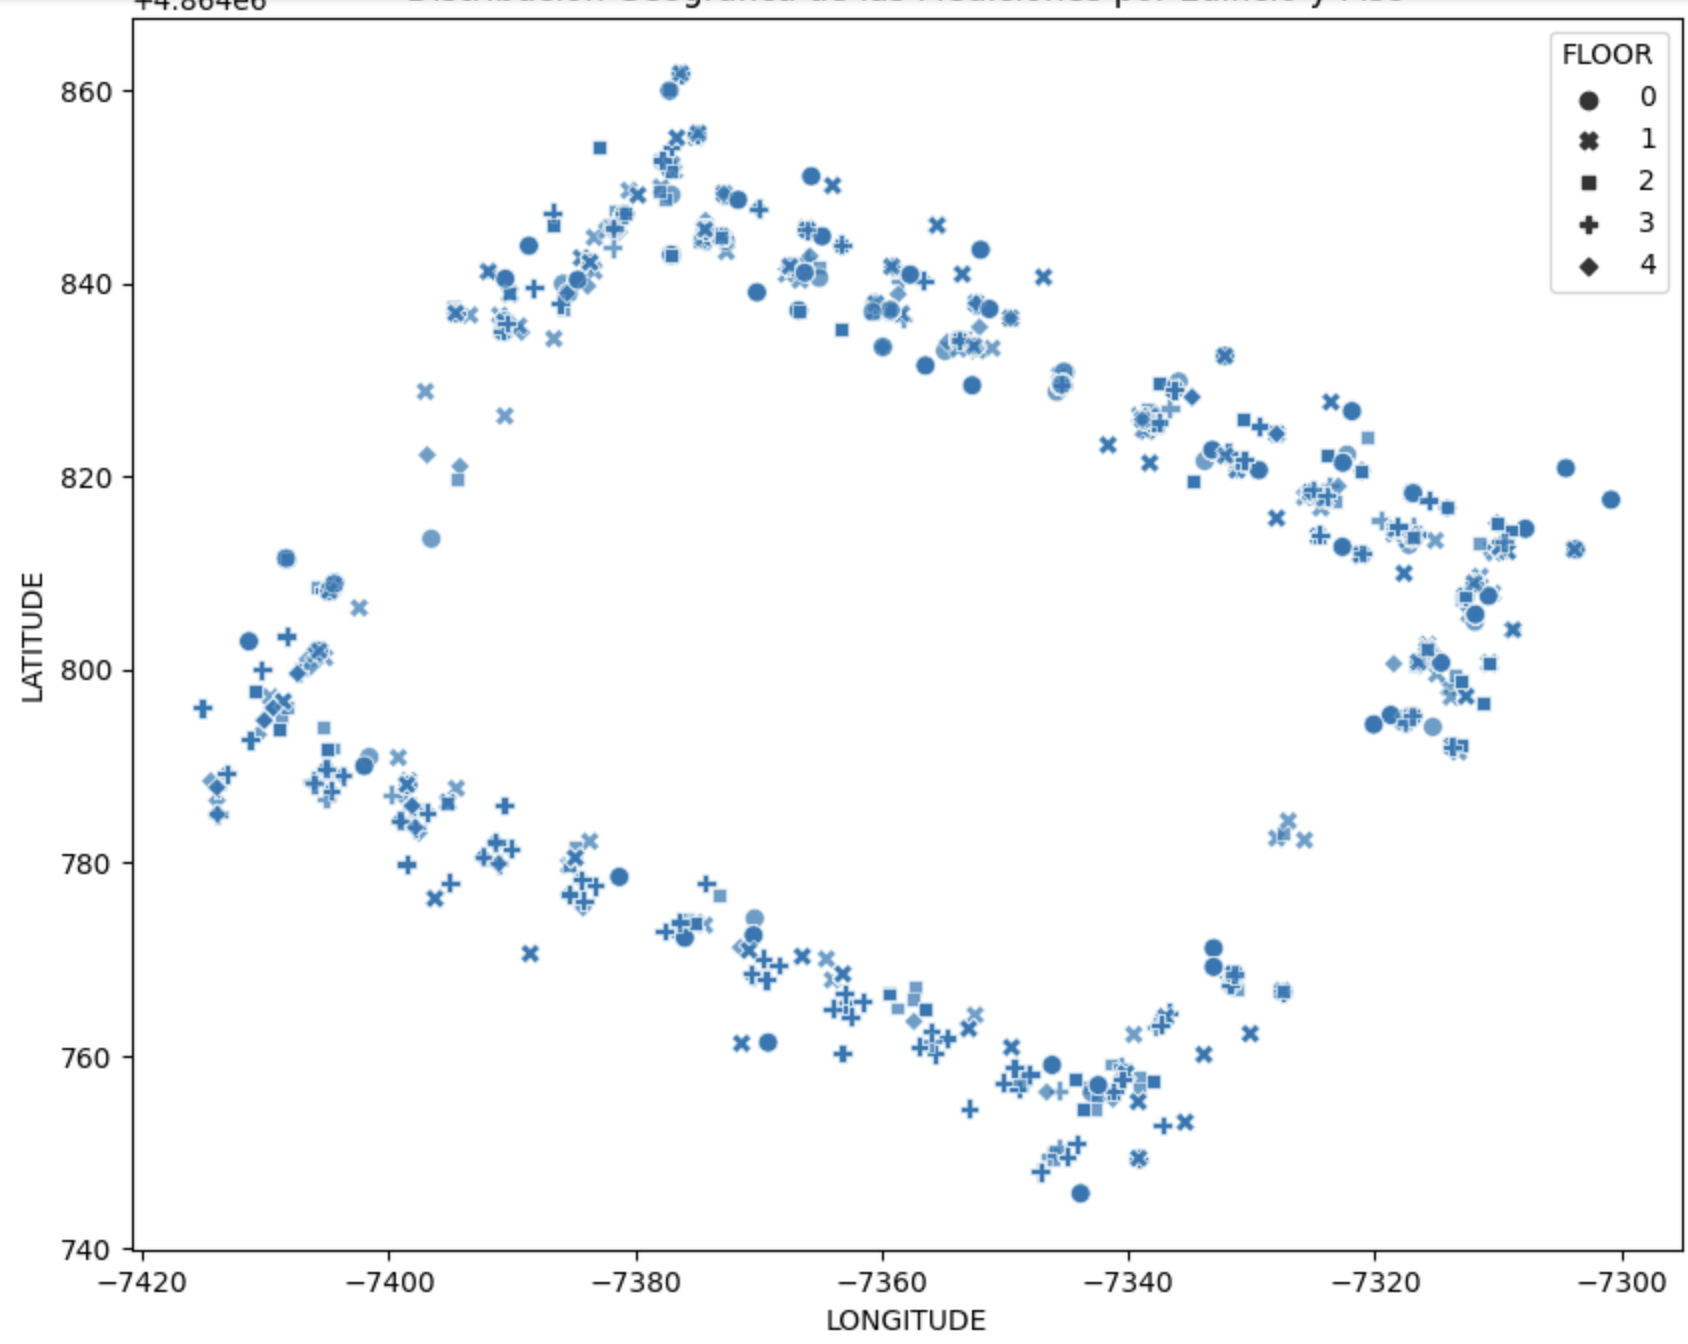
\includegraphics[width=0.5\linewidth]{Images/Image7.png}
    \caption{Geographical Measurement Distribution}
    \label{fig:enter-label}
\end{figure}


Finally, data normalization is performed using standard scaling, resulting in a standardized dataset for model development. This normalization process ensures that all variables have similar scales, enhancing model performance and interpretability.

\section{Development and Analysis}

Following the acquisition and processing of the initial data, a series of crucial steps were undertaken to optimize the dataset for machine learning models.

\subsection{Normalization and Data Grouping}

Initially, data were grouped based on spaces, identified by the \textit{SPACEID} column. This grouping allowed for better normalization and data segmentation. The \textit{SPACEID} column was temporarily removed, and a k-means clustering algorithm with four clusters was used in its place to identify and label similar groups based on latitude and longitude.

Subsequently, standard data normalization was performed. Numeric variables were standardized to have a mean of 0 and a standard deviation of 1, while categorical variables (such as \textit{FLOOR} and clusters derived from \textit{SPACEID}) were encoded using one-hot encoding. This transformation converted categories into binary columns, facilitating their use in machine learning models.

\subsection{Data Split}

Once processed, the data were divided into predictor variables "X" and target variables "y". Predictor variables excluded latitude and longitude coordinates, as well as categories derived from floor and space, while target variables focused on these coordinates and categories.

\section{Model Analysis}

\subsection{RandomForestRegressor Model}

\textbf{Method}: A RandomForestRegressor model was employed, consisting of 200 trees and utilizing 10 parallel jobs. The tree depth limit was set to 10.

\textbf{Results}:
\begin{itemize}
    \item Mean Squared Error (MSE): $0.01778$
    \item Root Mean Squared Error (RMSE): $0.13336$
    \item Mean Absolute Error (MAE): $0.05220$
    \item Coefficient of Determination $R^2$: $0.94$
\end{itemize}

\textbf{Interpretation}: The RandomForestRegressor model showcases a high degree of accuracy, with an $R^2$ value of $0.94$, indicating its ability to explain 94\% of the variability in the training data. The MSE, RMSE, and MAE metrics are comparatively low, suggesting the model's solid performance on the training set.

\subsection{SVM Model}

\textbf{Method}: An SVM model with a polynomial kernel was employed.

\textbf{Results}:
\begin{itemize}
    \item Mean Squared Error (MSE): $0.02059$
    \item Root Mean Squared Error (RMSE): $0.14351$
    \item Mean Absolute Error (MAE): $0.08619$
    \item Coefficient of Determination $R^2$: $0.93$
\end{itemize}

\textbf{Interpretation}: The SVM model demonstrates slightly lower accuracy compared to the RandomForestRegressor, with an $R^2$ of $0.93$. However, it remains a robust model, capable of explaining 93\% of the variability in the training data. While its MSE and RMSE are marginally higher than the RandomForestRegressor model, they still lie within an acceptable range.

\subsection{Dense Neural Network}

\textbf{Method}: A dense neural network was designed, featuring the following architecture:
\begin{itemize}
    \item An input layer with 53 neurons, corresponding to the dataset's 53 features.
    \item Four hidden layers with 240 neurons each, interleaved with \textit{Dropout} layers set at 20\% to prevent overfitting.
    \item A hidden layer of 120 neurons followed by \textit{Dropout} layers at 20\%, and an additional layer of 60 neurons.
    \item An output layer consisting of 11 neurons, representing the 11 prediction features for user localization.
\end{itemize}

The model was compiled using the Adam optimizer and a loss function based on the mean squared error (MSE). The metric used to assess performance during training was binary accuracy.

\textbf{Results}:
\begin{itemize}
    \item Mean Squared Error (MSE): $0.02688$
    \item Root Mean Squared Error (RMSE): $0.16394$
    \item Mean Absolute Error (MAE): $0.05477$
    \item Coefficient of Determination $R^2$: $0.95$
\end{itemize}

\begin{figure}[h]
    \centering
    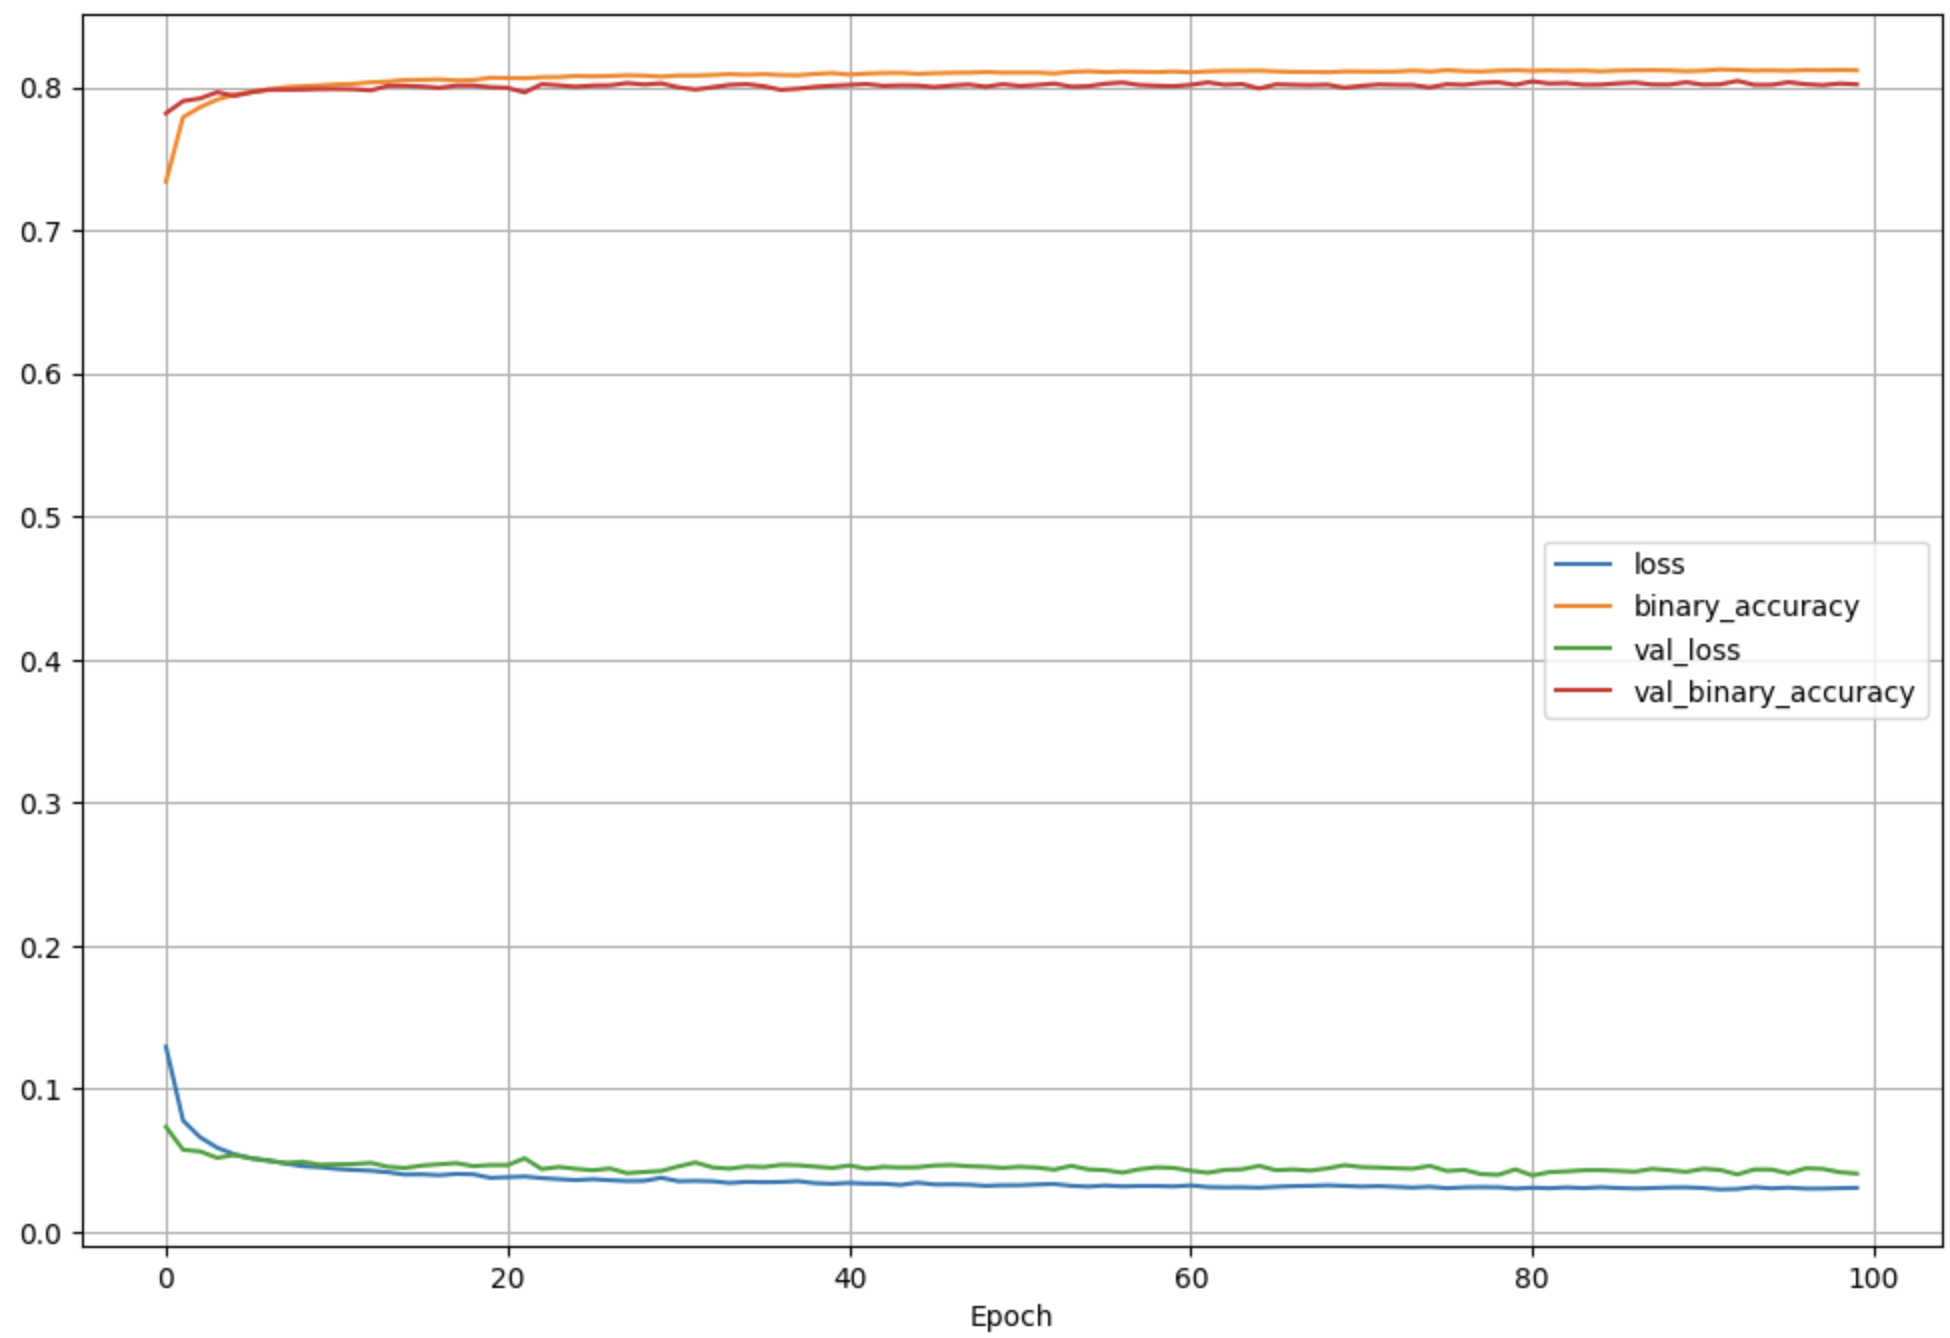
\includegraphics[width=0.5\linewidth]{REDNEURONAL1.png}
    \caption{Training evolution of the dense neural network}
    \label{fig:nn_training_evolution}
\end{figure}

\textbf{Interpretation}: The dense neural network displays a high degree of accuracy with an $R^2$ of $0.95$, denoting its ability to explain 95\% of the variability in the training data. The MSE, RMSE, and MAE metrics suggest a solid performance of the model on the training data. Figure \textcolor{blue}{\ref{fig:nn_training_evolution}} showcases a stable evolution of the training metrics, reflecting effective learning and potential early convergence of the model.

\subsection{Comparison and Conclusion}

Upon evaluating and comparing the three models, the following observations were made:
\begin{itemize}
    \item The \textbf{RandomForestRegressor} model exhibits an $R^2$ of $0.94$, indicating its capability to account for 94\% of the variability in the training data.
    \item The \textbf{SVM} model reports an $R^2$ of $0.93$, suggesting it's marginally less accurate when juxtaposed with the RandomForestRegressor but still stands as a high-performing model.
    \item The \textbf{Dense Neural Network} emerges as the top performer with an $R^2$ of $0.95$, underscoring its adeptness at capturing complex relationships within the dataset.
\end{itemize}

\textbf{Conclusion}: All three models display a high degree of accuracy in predicting localization features. The Dense Neural Network appears to be the most efficient, closely followed by the RandomForestRegressor. Although the SVM is slightly less accurate compared to the other two models, it still offers robust performance.

\section{Execution and Model Evaluation on Test Data}

\subsection{Storage and Loading of Models}

Four models, which had been previously developed, were stored and subsequently loaded for evaluation on test data. These models are K-means, Random Forest Regressor, SVM, and a Dense Neural Network.

\subsection{Test Data Pre-processing}

An independent copy of the test data was created to ensure that the original data remained unaltered throughout the process.

For spatial characterization, the previously trained K-means model was employed to predict the \texttt{SPACEID\_cluster} variable on the test data. This prediction categorizes areas within the dataset into specific clusters, simplifying their representation.

\begin{figure}[h]
    \centering
    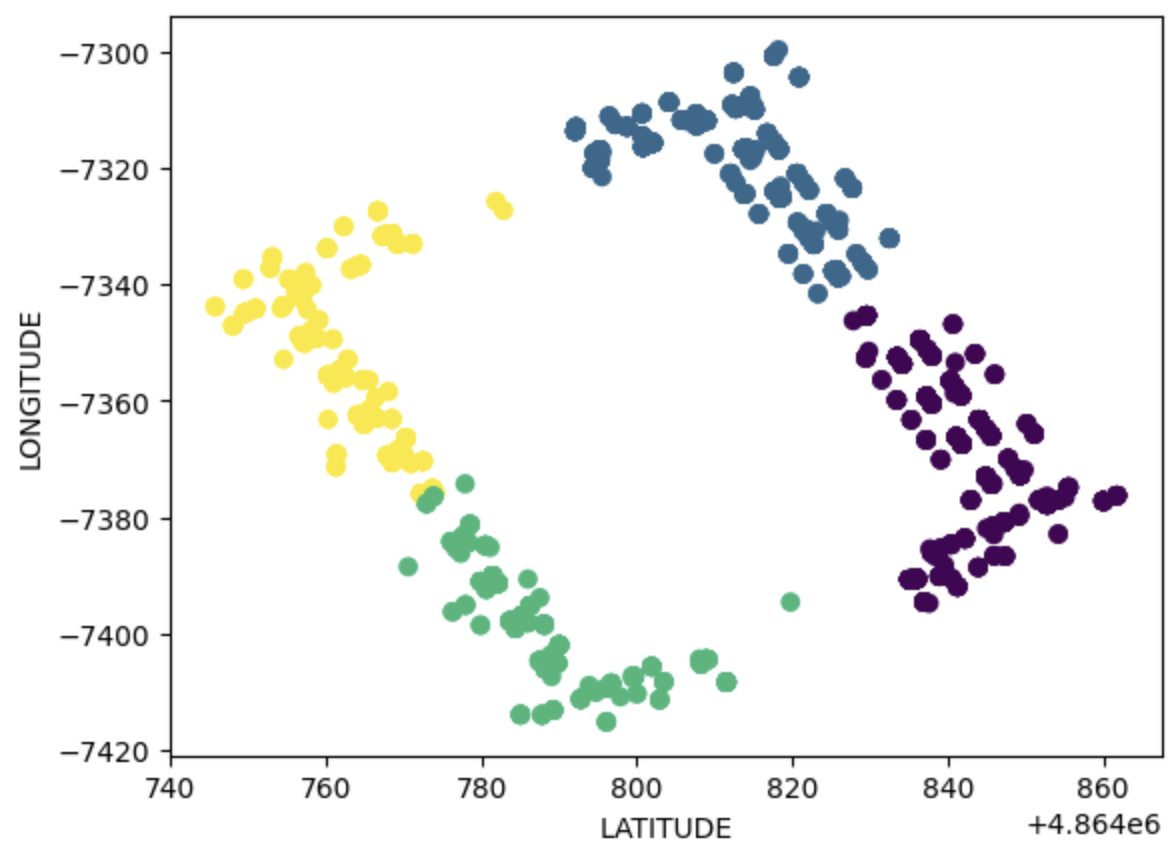
\includegraphics[width=0.7\linewidth]{procesamientoypruebadatos.png}
    \caption{Cluster distribution generated by k-means on test data.}
    \label{fig:clusters_test_data}
\end{figure}

\subsection{Standardization and One-hot Encoding}

Aiming to prepare data for the models, standardization and encoding techniques were employed. The data were standardized to maintain a uniform range and scale, which eases the training and evaluation processes for the models. Categorical variables, notably \texttt{FLOOR} and \texttt{SPACEID\_cluster}, were encoded using the one-hot method, thereby converting these categories into more manageable binary formats for the models.

\subsection{Data Split}

Relevant features and labels were identified and segregated for evaluation. The features, denoted as \texttt{X}, encompass information about Wi-Fi signal strength and other pertinent factors. The labels, denoted as \texttt{y}, represent the physical location, such as latitude, longitude, and the specific floor of the building. These prepared sets are directly used in the models to evaluate their accuracy and performance.

\section{Evaluation of Models on Test Data}

With the prepared test data, we proceeded to evaluate the performance of three models: RandomForest, SVM (Support Vector Machine), and Dense Neural Network. The performance of each model is gauged using four metrics: Mean Squared Error (MSE), Root Mean Squared Error (RMSE), Mean Absolute Error (MAE), and the coefficient of determination \( R^2 \).

\subsection{RandomForest}

The RandomForest model reported the following metrics:

\begin{itemize}
    \item Mean Squared Error (MSE): 0.03287
    \item Root Mean Squared Error (RMSE): 0.18130
    \item Mean Absolute Error (MAE): 0.07531
    \item \( R^2 \): 0.89
\end{itemize}

\textbf{Result Analysis:}
The RandomForest model exhibited solid predictive capability, with a determination coefficient \( R^2 \) of 0.89. This indicates the model's ability to explain 89\% of the data variability. The RMSE, which sheds light on the average prediction error, is reasonably low.

\subsection{SVM (Support Vector Machine)}

The SVM model's performance metrics are:

\begin{itemize}
    \item Mean Squared Error (MSE): 0.03601
    \item Root Mean Squared Error (RMSE): 0.18975
    \item Mean Absolute Error (MAE): 0.11176
    \item \( R^2 \): 0.87
\end{itemize}

\textbf{Result Analysis:}
The SVM model's performance is slightly inferior compared to the RandomForest model. While its \( R^2 \) remains high, its MAE is larger, suggesting that the SVM model predictions, on average, are farther from actual values than those of the RandomForest model.

\subsection{Dense Neural Network}

The performance metrics for the Dense Neural Network are:

\begin{itemize}
    \item Mean Squared Error (MSE): 0.04196
    \item Root Mean Squared Error (RMSE): 0.20484
    \item Mean Absolute Error (MAE): 0.07024
    \item \( R^2 \): 0.89
\end{itemize}

\textbf{Result Analysis:}
The Dense Neural Network's performance is comparable to the RandomForest model in terms of \( R^2 \). However, its RMSE is higher, signifying that, on average, the model's predictions have a larger error. Despite this, the MAE is competitive, implying that the model's predictions are typically close to the actual values, but there might exist some significant outliers affecting the RMSE.

\section{Employment of Autoencoder}

To enhance feature selection and reduce dimensionality, we decided to employ an autoencoder. We started by making a copy of the data with which the prior models were trained, considering all WAP columns. The intent is to identify and extract the 53 most pertinent features using the autoencoder.

Moreover, it was observed that 59 records showcased inconsistencies in all WAP measurements. Such records might hinder optimal model training, hence they were removed.

\subsection{Autoencoder Creation}

The autoencoder is constructed as a neural network aimed at reducing data dimensionality, in this case, from all WAPs to 56 features. Below is the neural network architecture utilized:

\begin{lstlisting}
Model:
- Input layer with 520 nodes
- Dense layer with 250 nodes and ReLU activation function
- Dense layer with 125 nodes and ReLU activation function
- Dense layer of 56 nodes (encoded features) with ReLU activation function
- Decoding layers with a similar but reverse structure
\end{lstlisting}


The autoencoder is compiled using the Adam optimizer and trained with mean squared error (MSE). The latent features are subsequently predicted and extracted for future use.

Upon employing k-means on latitude and longitude coordinates, the cluster distribution is visualized:

\begin{figure}[h]
\centering
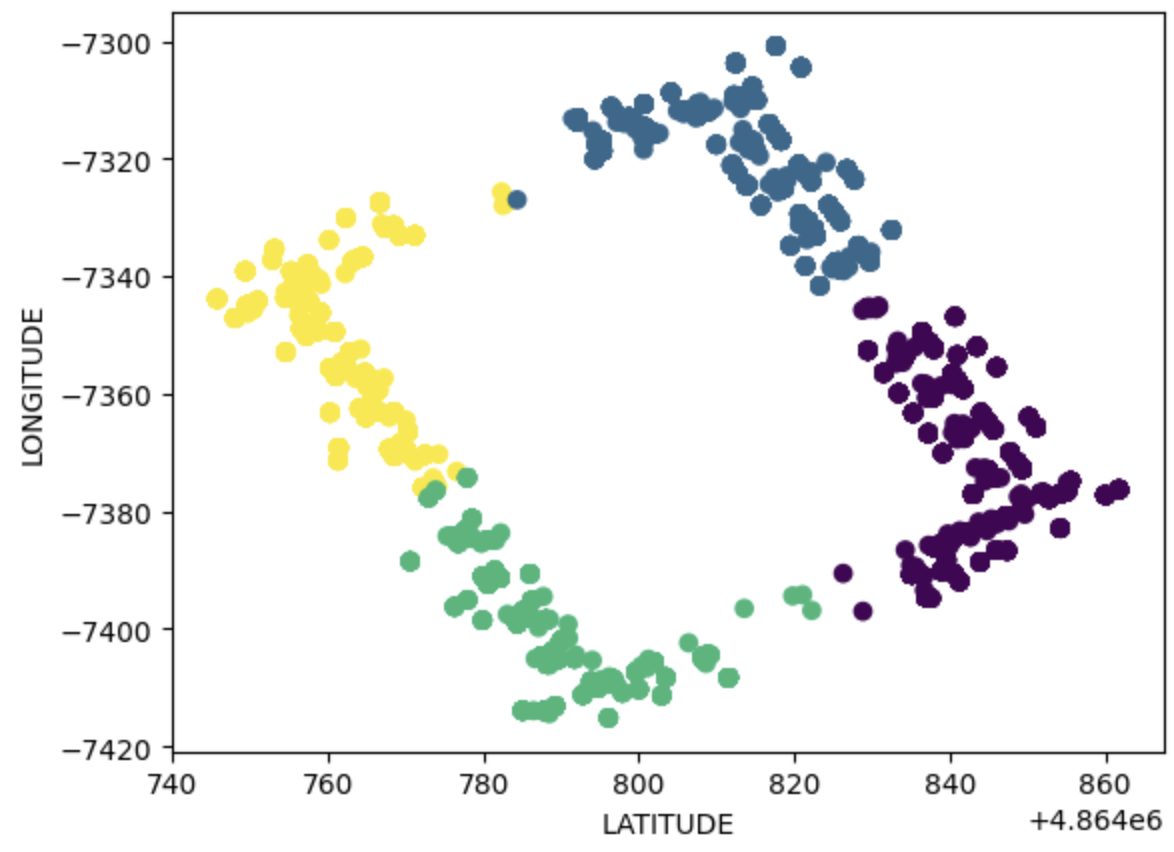
\includegraphics[width=0.5\linewidth]{imageau1.png}
\caption{Cluster distribution produced by k-means.}
\end{figure}

\subsection{Construction of Convolutional Model}

With the acquired features, a convolutional model is built. The model's architecture is as follows:

\begin{lstlisting}
Model:
- 1D Convolutional layer: 32 filters, 4 kernel size
- MaxPooling layer
- 1D Convolutional layer: 64 filters, 4 kernel size
- MaxPooling layer
- 1D Convolutional layer: 128 filters, 4 kernel size
- MaxPooling layer
- Flatten layer
- Successive dense layers of 200, 200, and 100 nodes
- Output layer with 11 nodes
\end{lstlisting}

The model is trained over 100 epochs, and the loss and accuracy evolution is visualized:

\begin{figure}[h]
\centering
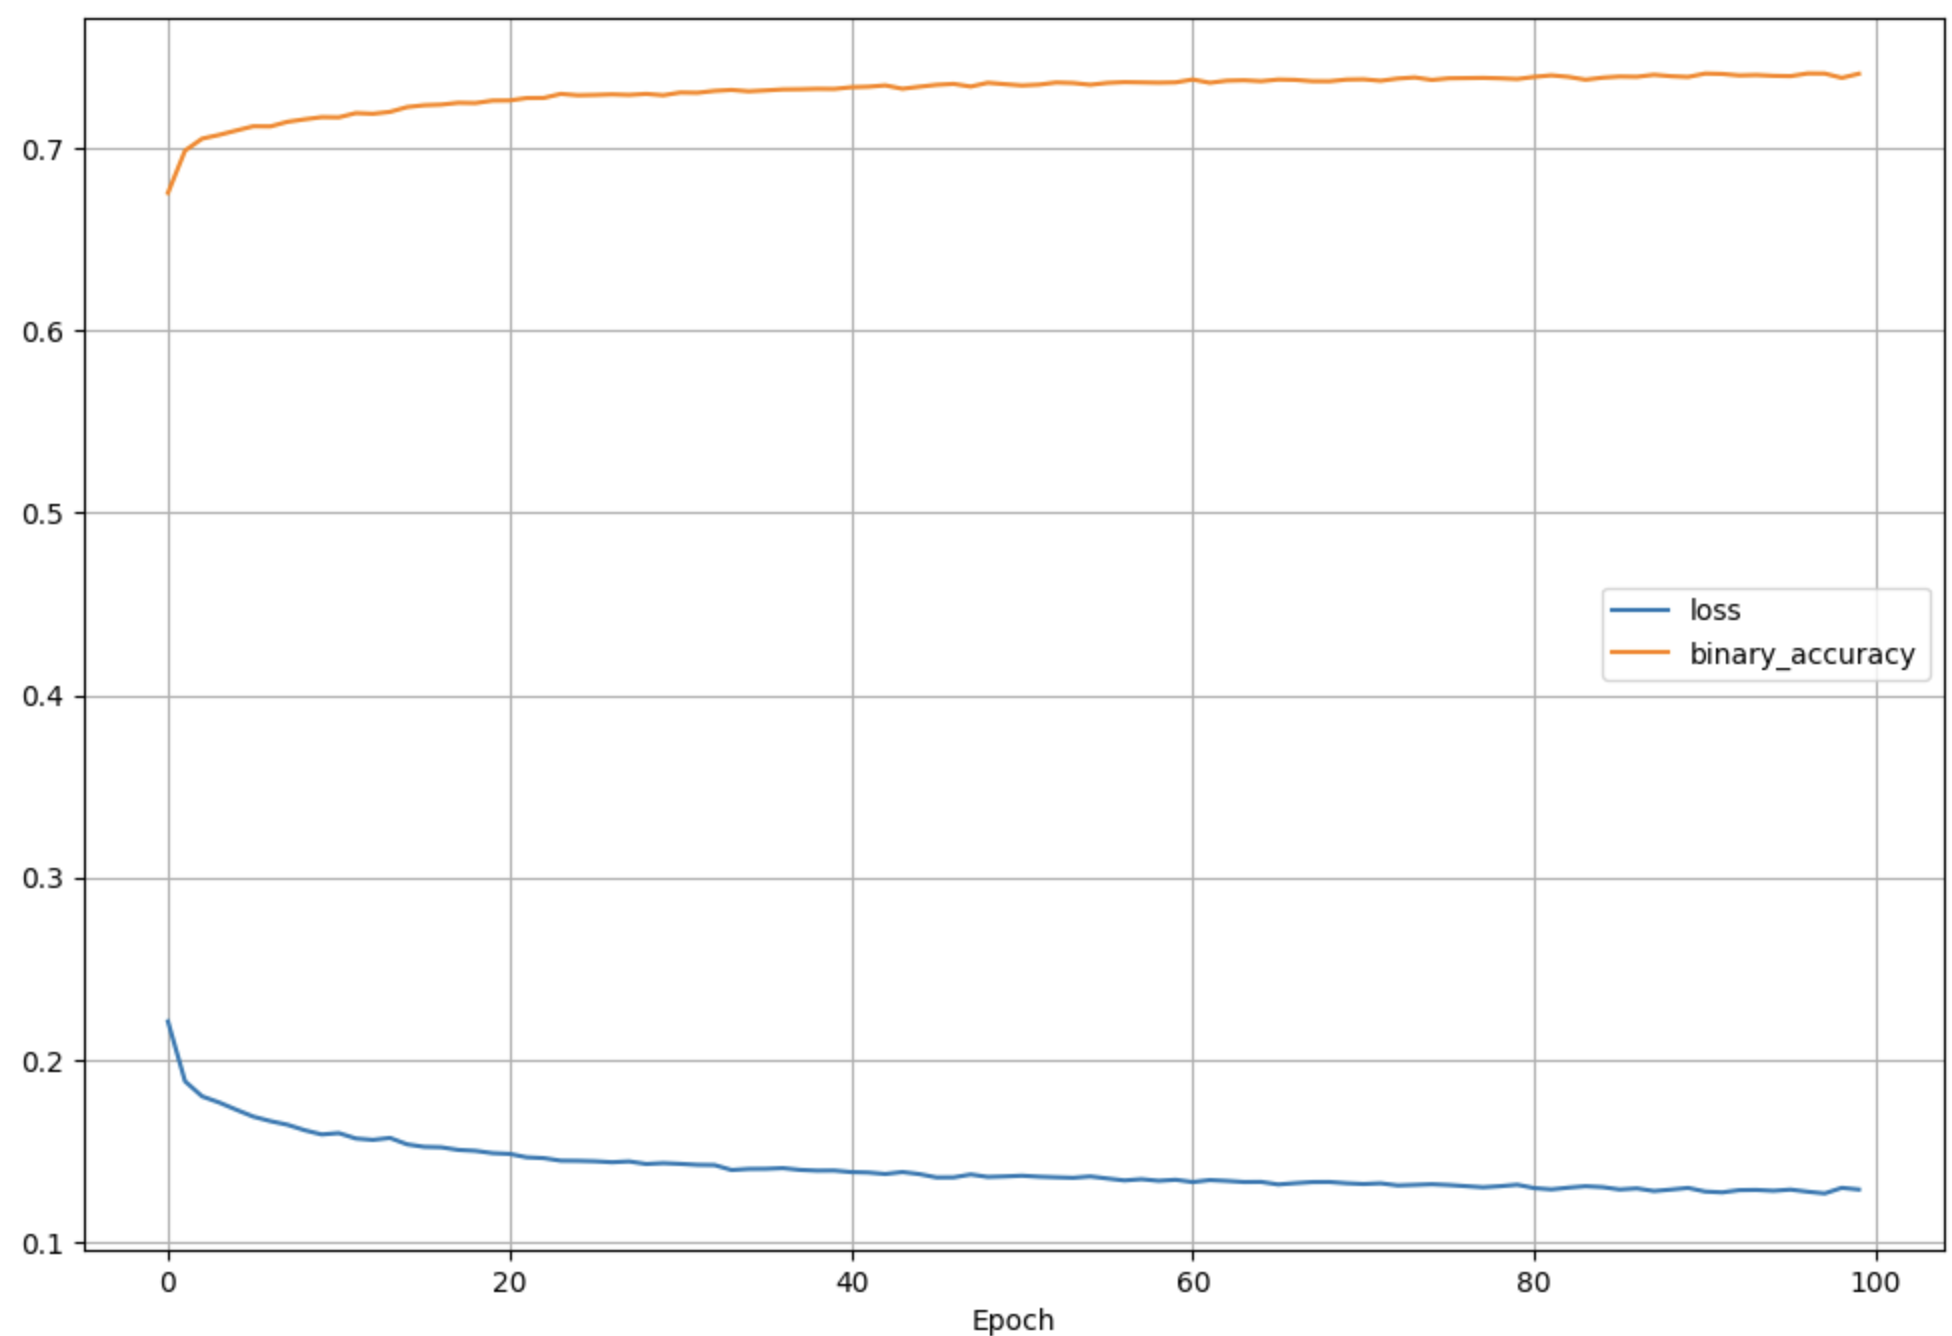
\includegraphics[width=0.5\linewidth]{imageau2.png}
\caption{Evolution of convolutional model's loss and accuracy.}
\end{figure}

\subsection{Convolutional Model Evaluation}

The model's metrics are as follows:

\begin{itemize}
    \item Mean Squared Error (MSE): 0.14123
    \item Root Mean Squared Error (RMSE): 0.37580
    \item Mean Absolute Error (MAE): 0.21563
    \item \( R^2 \): 0.55
\end{itemize}

\textbf{Result Analysis:}
The convolutional model, despite its intricate architecture, reports an \( R^2 \) of 0.55. This suggests room for improvement in its predictive capability. Additional adjustments in architecture or the training process might be needed to enhance its performance.

\section*{Conclusion}

In this research, we delved deep into an exhaustive analysis of the UJIIndoorLoc dataset, with the objective of uncovering valuable insights related to WLAN fingerprinting and indoor localization. Our meticulous examination shed light on multiple facets of the dataset, ranging from spatial distributions and attributes to the relevance and correlations of features.

Our initial visual interpretations unveiled critical insights. We observed that only one building showcased measurements on the fourth floor, insinuating the possible nonexistence of such a floor in other buildings. Our deductions also zeroed in on the notable skewness and high kurtosis of WAP measurements, with more than 90\% of data points registering a reading of -104 dBm. Additionally, we discerned that specific spaces (like rooms) housed a dominant concentration of measurements, pointing towards potential imbalances in data representation across locations.

Several machine learning models were trained and rigorously evaluated on both training and test datasets. Notably, the Dense Neural Network stood out, reporting the highest \( R^2 \) value of 0.95, marking it as the best performer among all. SVM and RandomForest models also showcased commendable results, with the latter slightly outshining the former.

Our subsequent endeavor into leveraging an autoencoder to distill essential features and reduce data dimensionality was insightful. The convolutional model constructed post feature extraction, however, exhibited a mediocre \( R^2 \) value, implying potential optimization opportunities.

In sum, our deep-dive into the UJIIndoorLoc dataset and consequent model evaluations offer a comprehensive overview of indoor localization methodologies based on WLAN fingerprinting. This research paves the way for future explorations and augmentations in the realm of indoor positioning systems.


\\

You can find the GitHub repository here: \href{https://github.com/ccamachosa31/IAProyectoDL}{GitHub Repository}.


\bibliographystyle{unsrt}
 	\bibliography{Bibliography/referencias}
%Torres-Sospedra,Joaqun, Montoliu,Raul, Martnez-Us,Adolfo, Arnau,Tomar, and Avariento,Joan. (2014). UJIIndoorLoc. UCI Machine Learning Repository. https://doi.org/10.24432/C5MS59.

\vspace{12pt}

\end{document}
